\chapter{Extra Results}

\section{ByteNet}
\label{appendix:result:bytenet-profile}

\subsection{WMT NewsTest profiling using one GPU}
\begin{figure}[h]
    \centering
    \includegraphics[width=\textwidth]{bytenet/profile-raw-gpu1.png}
    \caption{Shows time spend on each operation, when the operation was executed, and on what GPU/CPU it was executed. The color coding indicates the operation type, there are more than a 100 different operation types, most are specific to TensorFlow, thus the legend is not included.}
\end{figure}

\begin{figure}[h]
    \centering
    \includegraphics[scale=1]{bytenet/profile-grouped-gpu1.pdf}
    \caption{Shows time spend executing each part of the ByteNet model, this excludes the waiting time. Each part exists in a hierarchy, which is visualized as levels. Bottom level is the backward and forward pass. Second level is the encoder and decoder. Last level primarily splits the SELU ByteNet Residual Blocks.}
\end{figure}

\clearpage

\section{Simplified ByteNet}
\label{appendix:result:bytenet-small}
\subsection{Learning Synthetic Digits Problem}
\begin{figure}[h]
    \centering
    \includegraphics[scale=1]{bytenet-small/validation-synthetic-digits.pdf}
    \caption{Shows misclassification rate and the cross entropy loss. For comparison a the attention model has a misclassification rate of 0.51. The exponential moving average used a forget factor of $0.2$.}
\end{figure}
\clearpage

\subsection{Memorizing WMT NewsTest}
\begin{figure}[h]
    \centering
    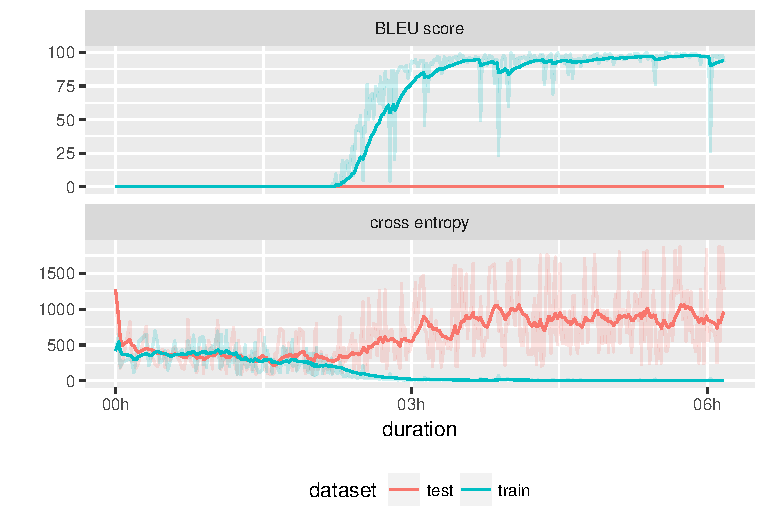
\includegraphics[width=\textwidth]{bytenet-small/validation-memorize-wmt.pdf}
    \caption{Shows BLEU score and cross entropy loss for the German to English WMT NewsTest dataset. Both training and test measures are calculated on a randomly sampled mini-batch from each dataset. The exponential moving average used a forget factor of $0.3$.}
\end{figure}
\clearpage

\subsection{WMT NewsTest profiling using four GPUs}
\begin{figure}[h]
    \centering
    \includegraphics[width=\textwidth]{bytenet-small/profile-raw-gpu4.png}
    \caption{Shows time spend on each operation, when the operation was executed, and on what GPU/CPU it was executed. The color coding indicates the operation type, there are more than a 100 different operation types, most are specific to TensorFlow, thus the legend is not included.}
\end{figure}
\clearpage


%\subsection{WMT NewsTest profiling using one GPU}
%\begin{figure}[h]
%    \centering
%    \includegraphics[width=\textwidth]{bytenet-small/profile-raw-gpu1.png}
%    \caption{Shows time spend on each operation, when the operation was executed, and on what GPU/CPU it was executed. The color coding indicates the operation type, there are more than a 100 different operation types, most are specific to TensorFlow, thus the legend is not included.}
%\end{figure}

%\begin{figure}[h]
%    \centering
%    \includegraphics[scale=1]{bytenet-small/profile-grouped-gpu1.pdf}
%    \caption{Shows time spend executing each part of the ByteNet model, this excludes the waiting time. Each part exists in a hierarchy, which is visualized as levels. Bottom level is the backward and forward pass. Second level is the encoder and decoder. Last level primarily splits the SELU ByteNet Residual Blocks.}
%\end{figure}

\clearpage

\section{SELU ByteNet}
\label{appendix:result:bytenet-selu}
\subsection{Learning Synthetic Digits Problem}
\begin{figure}[h]
    \centering
    \includegraphics[scale=1]{bytenet-selu/validation-synthetic-digits.pdf}
    \caption{Shows misclassification rate and the cross entropy loss. For comparison a the attention model has a misclassification rate of 0.51. The exponential moving average used a forget factor of $0.2$.}
\end{figure}

\clearpage
\subsection{WMT NewsTest profiling using four GPUs}
\begin{figure}[h]
    \centering
    \includegraphics[width=\textwidth]{bytenet-selu/profile-raw-gpu4.png}
    \caption{Shows time spend on each operation, when the operation was executed, and on what GPU/CPU it was executed. The color coding indicates the operation type, there are more than a 100 different operation types, most are specific to TensorFlow, thus the legend is not included.}
\end{figure}